\section{Κινητική}
Η εξαγωγή των εξισώσεων κίνησης έγινε με την εφαρμογή των νόμων του \tl{Euler}
\cite{natsiavas} για στερεό σώμα τόσο για τις μεταφορικές όσο και για τις 
περιστροφικές συνιστώσες του αεροχήματος. Οι εξισώσεις διατυπώνονται σε 
αδρανειακό σύστημα αναφοράς ως
\begin{gather}
    \mathbf{F} = \mathbf{(\dot L)}_{E} = m (\mathbf{{\dot v}}_G)_{E}
    \label{tmE1} \\
    \mathbf{M}_G = (\mathbf{{\dot H}}_G)_{E},
    \label{rmE}
\end{gather}
όπου \(\mathbf{F}\) η συνισταμένη εξωτερική δύναμη, που ασκείται στο σώμα,
\(\mathbf{L}\) η ορμή, \(m\) η συνολική μάζα του τρικοπτέρου και
\(\mathbf{{v}}_G\), η ταχύτητα του κέντρου μάζας του αεροχήματος. \(\mathbf{M}\),
η συνολική εξωτερική ροπή, που ασκείται στο σώμα, και \(\mathbf{H_G}\), η 
στροφορμή ως προς το κέντρο μάζας \(G\). Από εδώ κι στο εξής, η μεταφορική 
ταχύτητα του κέντρο μάζας ως προς το αδρανειακό σύστημα $(\mathbf{v}_G)_E$ θα 
σημειώνεται απλώς ως $\mathbf{v}$ και η γωνιακή ταχύτητα του αδρανειακού 
συστήματος αναφοράς ως προς το κεντροβαρικό σύστημα αναφοράς, εκφρασμένη στο 
κεντροβαρικό σύστημα $(\bm{\omega}_{B\!/E})_B$ σημειώνεται απλώς ως $\bm{\omega}
$.

Οι παραγώγιση της εξίσωσης (\ref{rmE}) επιλέγεται να γίνει στο κεντροβαρικό 
σύστημα αναφοράς καθώς προκύπτουν ορισμένα οφέλη. Ο τανυστής αδράνειας του 
σώματος παραμένει αμετάβλητος στο κεντροβάρικό σύστημα αναφοράς και, όπως 
αναφέρθηκε, οι άξονες των μετρητικών οργάνων συμπίπτουν με τους άξονες του 
συστήματος αναφοράς. Επιπλέον, το σύστημα κυρίων αξόνων του σώματος συμπίπτει με 
αυτό του κεντροβαρικού συστήματος αναφοράς πράγμα, που σημαίνει ότι τα μαζικά 
γινόμενα αδράνειας προκύπτουν αμελητέα σε σχέση με τις κύριες τιμές.

Η παράγωγος ενός διανύσματος \(\mathbf{q}\) εκφρασμένη σε ένα σύστημα \(f\) το
οποίο περιστρέφεται ως προς ένα σύστημα \(f'\) είναι
\begin{equation}
    (\mathbf{\dot q})_f = (\mathbf{\dot q})_{f'} + \bm{\omega}_{f'\!/f}
    \times \mathbf{q},
\end{equation}
όπου \(\bm{\omega}_{f'\!/f} \) η γωνιακή ταχύτητα του συστήματος \(f'\)
ως προς το \(f\).  Έτσι, παίρνουμε
\begin{gather*}
    % \mathbf{F}  = m \left((\mathbf{{\dot v}}_G)_{B} + \bm{\omega}
    % \times \mathbf{{\dot v}}_G\right) \label{tmB} \\
    \mathbf{M}_G = (\mathbf{{\dot H}}_G)_{B} + \bm{\omega}
    \times \mathbf{H}_G.
\end{gather*}
Η στροφορμή του σώματος ως προς το κεντροβαρικό σύστημα $( \mathbf{H}_G)_{B} = 
I_G \bm{\omega}$. Μιας και ο τανυστής αδράνειας παραμένει σταθερός, όντας 
υπολογισμένος στο κεντροβαρικό σύστημα, παίρνουμε
\begin{equation*}
    (\mathbf{\dot H}_G)_B = I_G \dot{\bm{\omega}}.
\end{equation*}

Στο σχήμα (\ref{fig:static_fbd}), που ακολουθεί, παρουσιάζεται το διάγραμμα
ελευθέρου σώματος του τρικοπτέρου. Εκεί, παρουσιάζονται τα φορτία που
προκύπτουν από τις έλικες καθώς και τα γεωμετρικά χαρακτηριστικά του
αεροχήματος. Οι δείκτες \(l,\, r,\, b\) αναφέρονται στον εμπρόσθιο αριστερά
$(\scriptstyle {x>0,\, y<0})_B$, εμπρόσθιο δεξιά $(\scriptstyle x>0,\,y>0)_B$ 
και οπίσθιο κινητήρα $(\scriptstyle x<0,\,y=0)_B$ αντίστοιχα. Ο ορισμός των
εκφράσεων των φορτίων των ελίκων γίνεται σε ξεχωριστή ενότητα μετέπειτα.

Οι δυνάμεις ώθησης \(\mathbf{T}_i\), για \(i\in\set{l, r, b}\), ορίζονται στο
κεντροβαρικό σύστημα συντεταγμένων κι έτσι, θα πρέπει να περιστραφούν για να
εκφραστούν στο αδρανειακό σύστημα. Το διάνυσμα της επιτάχυνσης της βαρύτητας 
$\mathbf{g}$ είναι εκφρασμένο εξαρχής στο αδρανειακό σύστημα αναφοράς, έτσι η 
συνισταμένη δύναμη παίρνει τη μορφή
\begin{equation}
    \mathbf{F}  = R \sum \mathbf{T}_i + m\mathbf{g}.
\end{equation}

Ορίζονται τα διανύσματα θέσης \(\mathbf{r}_i\) για \(i\in\set{l, r, b}\) των
σημείων άσκησης των φορτίων των προπελών ως προς το κέντρο μάζας εκφρασμένα στο 
κεντροβαρικό σύστημα. Οι διατυπώσεις, που προκύπτουν σύμφωνα με τα γεωμετρικά 
χαρακτηριστικά του σχήματος \ref{fig:static_fbd}, είναι
\begin{equation*}
    \mathbf{r}_l =
    \begin{pmatrix}
        {l_1 - l_4 sin(\theta_l)} \\
        {-l_3}                     \\
        {-l_4 cos(\theta_l)}
    \end{pmatrix}
    ,\quad \mathbf{r}_r =
    \begin{pmatrix}
        {l_1 - l_4 sin(\theta_r)} \\
        {l_3}                    \\
        {-l_4 cos(\theta_r)}
    \end{pmatrix}
    ,\quad \mathbf{r}_b =
    \begin{pmatrix}
        {-l_2} \\
        {0}    \\
        {0}
    \end{pmatrix},
\end{equation*}

\noindent όπου οι \(\theta_l\), \(\theta_r\) είναι οι γωνίες κεκλιμένου 
στροφείου, οι οποίες αποτελούν και μεταβλητές ελέγχου. Η θετική φορά των γωνιών 
είναι αυτή που φαίνεται στο σχήμα (\ref{fig:static_fbd}) και είναι στη διεύθυνση
του άξονα \(e_y\).

Οι ροπές αντίδρασης \(\mathbf{N}_i\), για \(i\in\set{l, r, b}\) έχουν φορά
αντίθετη από αυτή της περιστροφής των κινητήρων. Η κατεύθυνση τους φαίνεται στο
σχήμα (\ref{fig:static_fbd}). Όπως παρατηρεί κανείς, η φορά των δύο εμπρόσθιων 
κινητήρων είναι αντίθετη από την φορά του οπίσθιου. Η επιλογή αυτή έγινε ούτως 
ώστε η παραγόμενη συνισταμένη ροπή αντίδρασης να έχει το ελάχιστο μέτρο. Η 
συνεισφορά του κάθε κινητήρα στην συνισταμένη ροπή αποτελείται από τη ροπή, που 
δημιουργεί η δύναμη ώθησης και από την ροπή αντίδρασης. Η συνισταμένη ροπή ως 
προς το κέντρο μάζας του κινητήρα υπολογίζεται
\begin{equation}
    \mathbf{M}_G  =  \sum(\mathbf{r}_i \times \mathbf{T}_i + \mathbf{N}_i).
\end{equation}

Οι εξισώσεις κίνησης, που προκύπτουν, είναι
\begin{gather}
    m \mathbf{{\dot v}} = R \sum \mathbf{T}_i + m\mathbf{g}\label{knt:trans} \\ 
    I_G \dot{\bm{\omega}} = \mathbf{M}_G - \bm{\omega}\times{I_G\bm{\omega}}.
    \label{knt:rot}
\end{gather}

Στο σχήμα που ακολουθεί, παρουσιάζεται το διάγραμμα ελευθέρου σώματος. Η
γεωμετρία του τρικοπτέρου περιγράφεται πλήρως με ένα τρίγωνο του οποίου οι ακμές
είναι οι αρχικές θέσεις των κινητήρων. Έτσι, το διάγραμμα ελευθέρου σώματος 
έγινε σε αυτό το τρίγωνο για την αποφυγή περιττής πληροφορίας.

\begin{figure}[htb!]
    \centering
    \begin{tikzpicture}[scale=1]
        \tikzset{cross/.style={
                    cross out, draw=black, minimum size=2*(#1-\pgflinewidth),
                    inner sep=0pt, outer sep=0pt}, cross/.default={1pt}}
        \node[anchor=south west,inner sep=0] (image) at (0,0)
        {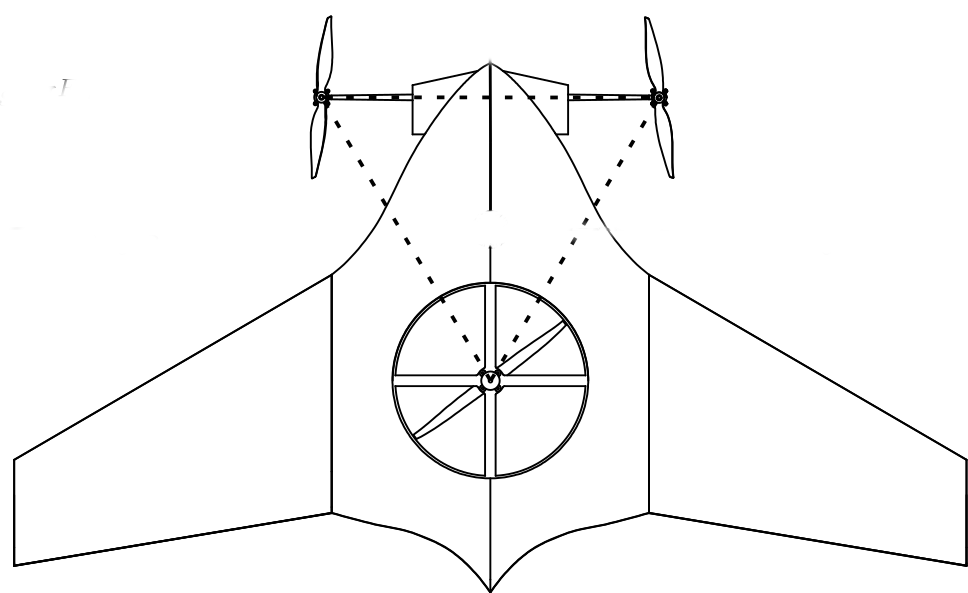
\includegraphics[scale=0.5]{Dynamics/FreeBodyDiagram1.png}};
        \draw[thick,-stealth] (6.5, 5) -- (6.5, 6) node[right] {\(e_x\)};
        \draw[thick] (6.5, 5) node[cross=4] {};
        \draw[thick] (6.5, 5) circle(4pt) node[left, outer sep=2.5] {\(e_z\)};
        \draw[thick] (6.5, 5) node[below right] {\(G\)};
        \draw[thick,-stealth] (6.5, 5) -- (7.5, 5) node[above] {\(e_y\)};
        \draw[very thick] (6.5, 5) -- (6.5, 4.1);
    \end{tikzpicture}
    % \caption{Διάγραμμα ελευθέρου σώματος.}\label{fig:static_fbd}
    % \end{figure}

    % \begin{figure}[!ht]%\kern-1.5ex
    \tikzset{cross/.style={
                cross out, draw=black, minimum size=2*(#1-\pgflinewidth),
                inner sep=0pt, outer sep=0pt}, cross/.default={1pt}}
    \centering
    \begin{tikzpicture}[scale=2.8]
        \draw[thick,dashed] (0.0, -0.2) -- (0.0, 2);
        \draw[thick,dashed] (0.0, 2.0) -- (-0.5, 2)
        node[above,pos=0.5] {\(l_4\)};
        \draw[thick,-stealth] (-0.5, 2.0) arc(180: 210: 0.5)
        node[left,pos=0.5] {\(\theta_l\)};;
        \draw[thick,dashed] (0.0, 2.0) -- (-0.43301, 2.0 - 0.25);
        \draw[thick,-stealth] (-0.43301, 2.0 - 0.25) --
        (-0.86603, 2 - 0.5) node[left] {\(T_l\)};
        \draw[thick,-{stealth}{stealth}] (-0.51962, 2.0 - 0.3)
        node[below,inner sep=6.0] {\(N_l\)} -- (-0.60622, 2.0 - 0.35);
        \draw[thick, -stealth] (-0.3, 2.0) arc(180: 245: 0.3)
        node[left] {\(\theta_r\)};
        \draw[thick,dashed] (0.0, 2.0) -- (-0.21131, 2.0 - 0.45315);
        \draw[thick,-stealth] (-0.21131, 2.0 - 0.45315) --
        (-0.42262, 2 - 0.90631)
        node[left] {\(T_r\)};
        \draw[thick,-{stealth}{stealth}] (-0.25357, 2.0 - 0.54378)
        node[below right,inner sep=1.0] {\(N_r\)} -- (-0.29583, 2.0 - 0.63442);
        % \draw[thick,-{stealth}{stealth}] (-0.29583, 2.0 - 0.63442)
        % node[right,outer sep=1.0] {\(N_r\)} -- (-0.25357, 2.0 - 0.54378);
        \draw[thick,dashed] (-0.43301, 2.0 - 0.25) arc(210: 270: 0.5);

        \draw[thick,-stealth] (0.0, 0.8) -- (0.0, 1.3) node[right] {\(e_x\)};
        \draw[fill] (0.0, 0.8) circle(0.5pt) node[left,outer sep=2] {\(e_y\)};
        \draw[fill] (0.0, 0.8) node[below right] {\(G\)};
        \draw (0.0, 0.8) circle(1.5pt);
        \draw[thick,-stealth] (0.0, 0.8) -- (0.5, 0.8) node[right] {\(e_z\)};

        \draw[thick,-stealth] (0.0, -0.2) -- (-0.5, -0.2)
        node[left] {\(T_b\)};
        \draw[thick,-{stealth}{stealth}] (-0.2, -0.2) -- (-0.1, -0.2)
        node[below] {\(N_b\)};

        \draw[thick] (2.0, -0.2) -- (1.0, 2.0) -- (3.0, 2.0) -- (2.0, -0.2);
        \draw (1.5, 2.0) node[below] {\(l_3\)};
        \draw[thick,dashed] (2.0, -0.2) -- (2.0, 2.0);
        \draw (2.0, 0.6) node[left] {\(l_2\)};
        \draw (2.0, 1.7) node[left] {\(l_1\)};

        \draw[thick,-stealth] (2.0, 0.8) -- (2.0, 1.3) node[right] {\(e_x\)};
        \draw[thick] (2.0, 0.8) node[cross=3.4] {};
        \draw (2.0, 0.8) circle(1.5pt) node[left, outer sep=2.5] {\(e_z\)};
        \draw (2.0, 0.8) node[below right] {\(G\)};
        \draw[thick,-stealth] (2.0, 0.8) -- (2.5, 0.8) node[right] {\(e_y\)};

        \draw[fill] (2.0, -0.2) circle(0.5pt);
        \draw (2.0, -0.2) circle(1.5pt) node[below right] {\(T_b\)};
        \draw[thick, -stealth] (1.8121, -0.13160) arc(160: 20: 0.2)
        node[right,inner sep=1.0] {\(N_b\)};

        \draw[fill] (1.0, 2.0) circle(0.5pt);
        \draw (1.0, 2.0) circle(1.5pt) node[above right] {\(T_l\)};
        \draw[thick, -stealth] (1, 2.2) arc(90: 235: 0.2)
        node[below] {\(N_l\)};

        \draw[fill] (3.0, 2.0) circle(0.5pt);
        \draw (3.0, 2.0) circle(1.5pt) node[above left] {\(T_r\)};
        \draw[thick, -stealth] (3.0, 1.8) arc(-90: 50: 0.2)
        node[above,inner sep=5.0] {\(N_r\)};
    \end{tikzpicture}
    \caption{Διάγραμμα ελευθέρου σώματος.}\label{fig:static_fbd}
\end{figure}